\documentclass[12pt]{article}
\usepackage[margin=1in]{geometry} 
\usepackage{amsmath,amsthm,amssymb,amsfonts}
\usepackage{graphicx}
 
\newcommand{\N}{\mathbb{N}}
\newcommand{\Z}{\mathbb{Z}}
 
\newenvironment{problem}[2][Problem]{\begin{trivlist}
\item[\hskip \labelsep {\bfseries #1}\hskip \labelsep {\bfseries #2.}]}{\end{trivlist}}
%If you want to title your bold things something different just make another thing exactly like this but replace "problem" with the name of the thing you want, like theorem or lemma or whatever

\newenvironment{answer}[2][Answer]{\begin{trivlist}
\item[\hskip \labelsep {\bfseries #1}\hskip \labelsep {\bfseries #2.}]}{\end{trivlist}}

\begin{document}
 
%\renewcommand{\qedsymbol}{\filledbox}
%Good resources for looking up how to do stuff:
%Binary operators: http://www.access2science.com/latex/Binary.html
%General help: http://en.wikibooks.org/wiki/LaTeX/Mathematics
%Or just google stuff
 
\title{AST 221: Problem Set 3}
\author{Your Name Goes Here}
\maketitle

\noindent {\bf Due: Thursday, Feb. 28 by midnight.} Late papers are not accepted after Feb. 28 (midnight). If you cannot complete the assignment by then, hand in what you have completed before the deadline. Consider the deadline to be like the boarding time for an airplane, or the deadline for a grant submission to NASA or NSF. If you miss the deadline, you do not get on the airplane, no matter how good your excuse is. If you miss an NSF or NASA deadline, you do not get the grant, no matter how good your project is. The best advice is ... finish early. You can submit multiple times, right up to the deadline. Whatever your latest submission is, when the deadline occurs, is what will be graded.
 
\begin{problem}{1} There is an error in the book on page 108? What correction is required?

\end{problem}

\begin{answer}{1}
Your answer goes here. Show your work. Justify your conclusions.
\end{answer}

\begin{problem}{2} Become familiar enough with stellar spectra that you can easily classify, at a glance, almost any spectrum into one of the main classes (OBAFGKM) to within plus or minus 1 class. Note that I am not talking about subclasses here, i.e telling a G2 star from a G3 star, which is difficult. I am talking about telling a G star from an A star or an M star. As an illustration of your prowess, how would you classify each of the stars shown below.

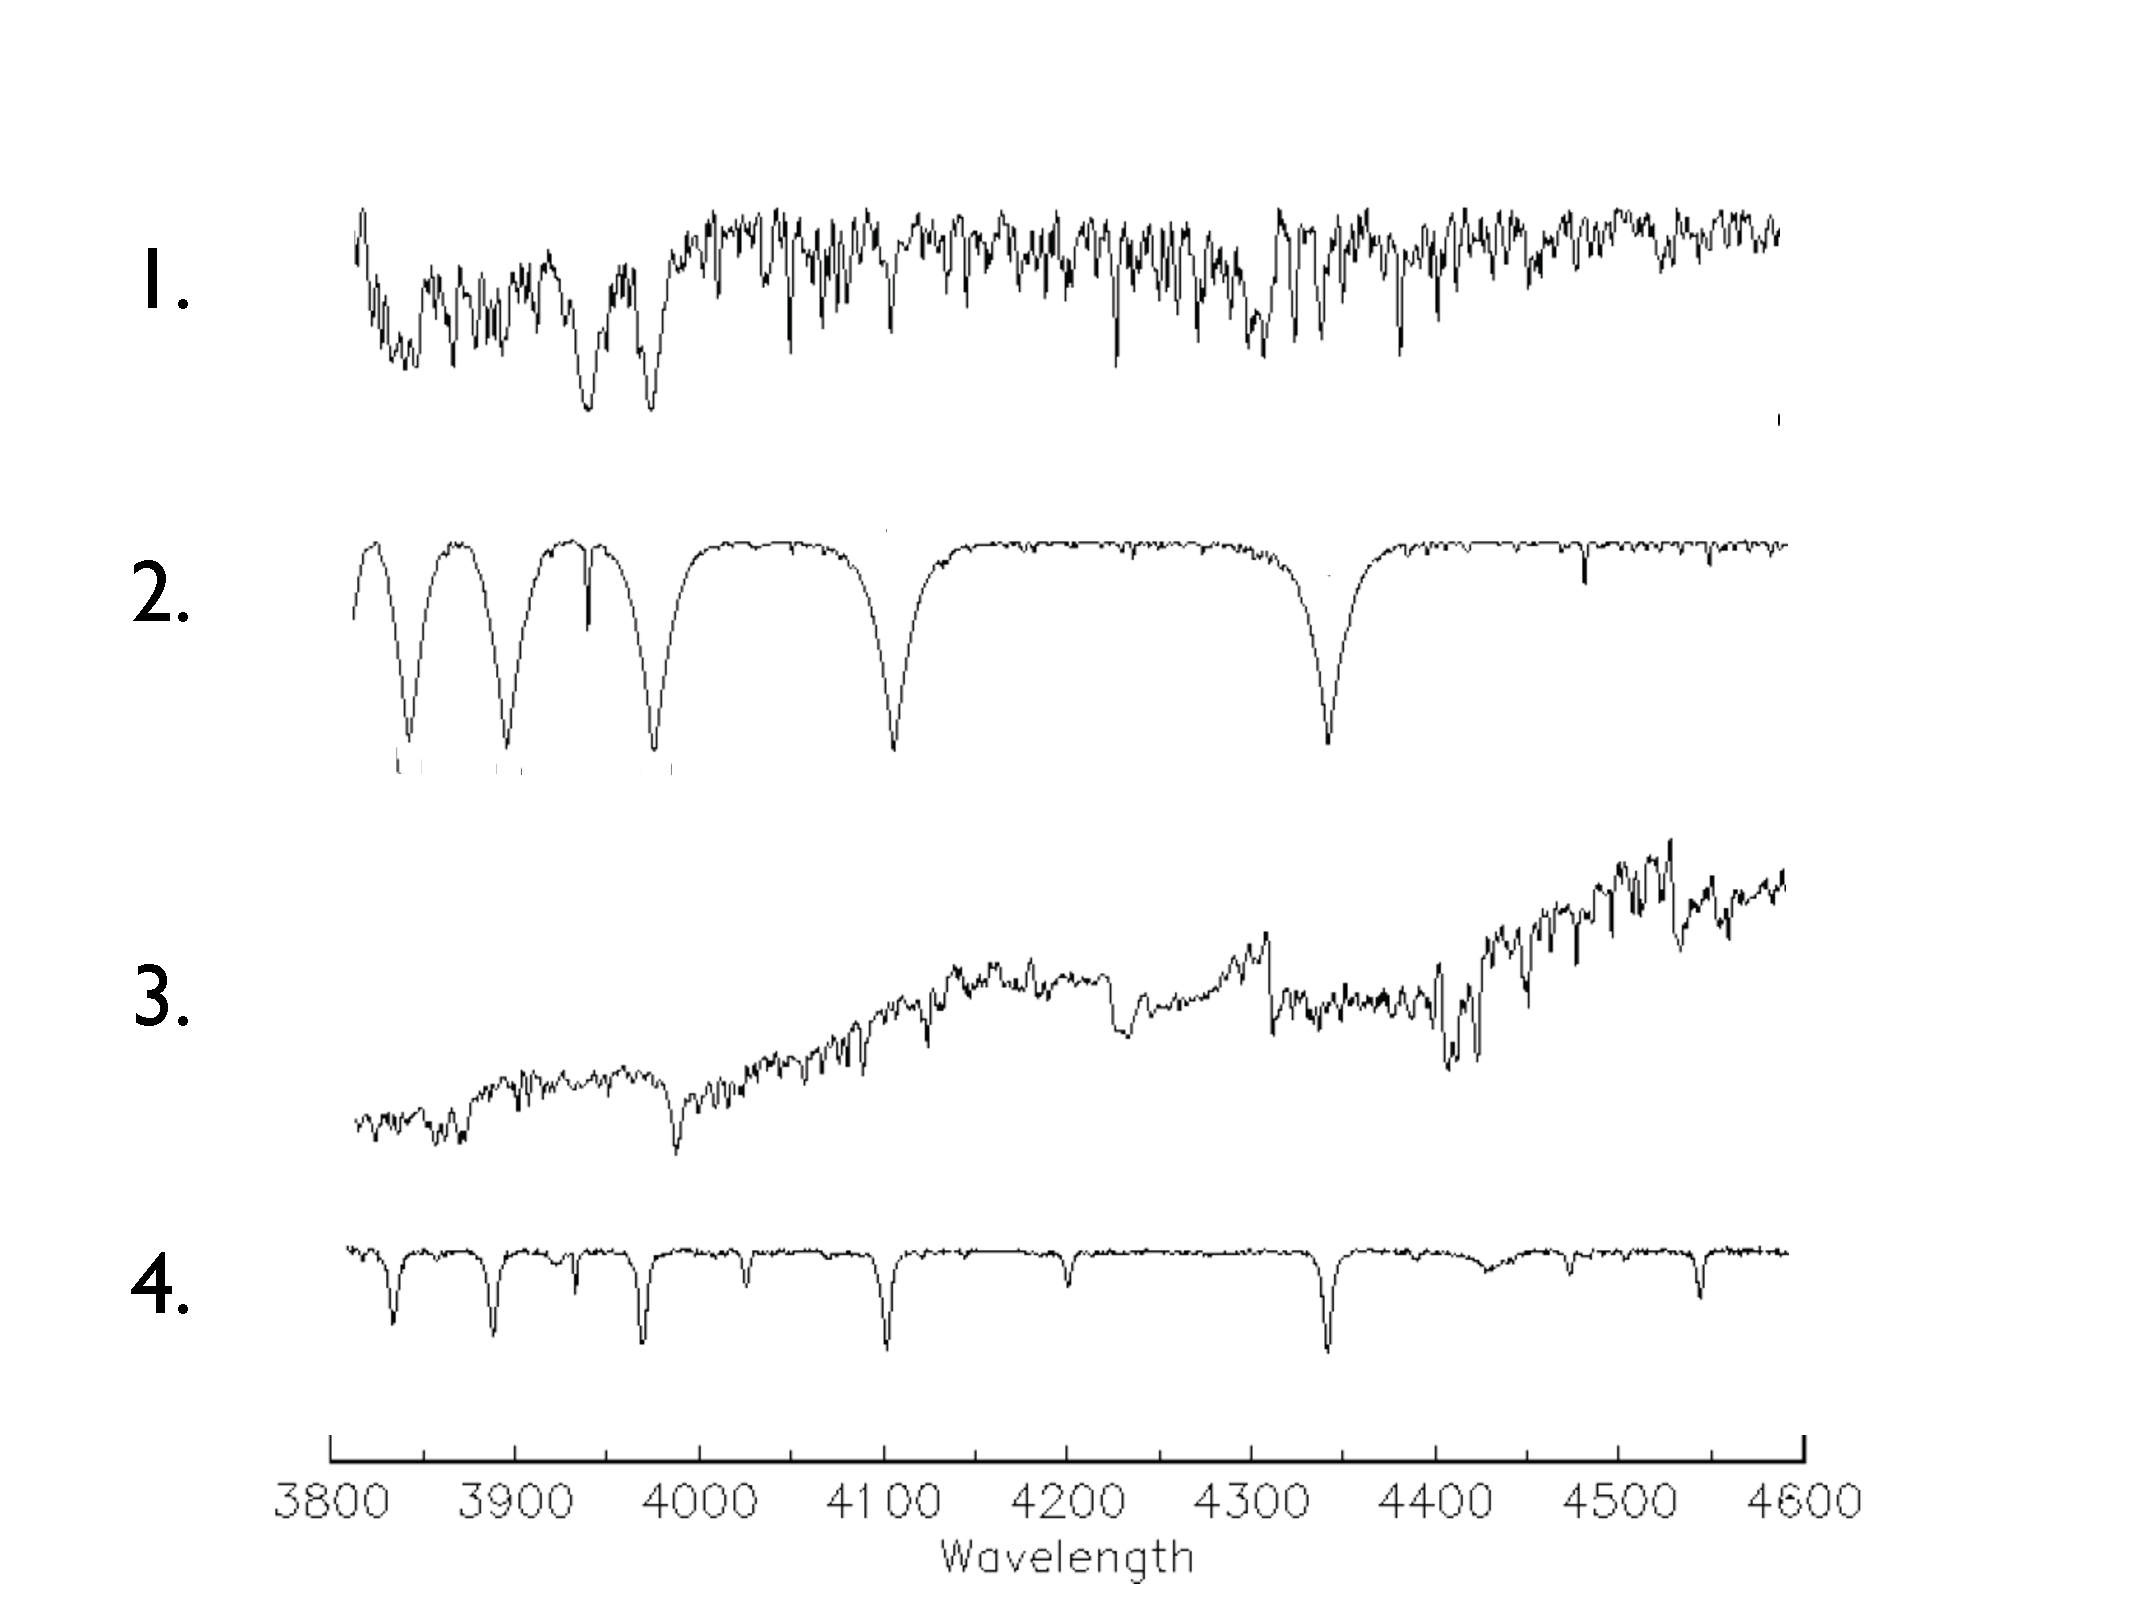
\includegraphics [scale=0.3] {UnknownSpectra.pdf}

\end{problem}

\begin{answer}{2}
Your answer goes here. Show your work. Justify your conclusions.
\end{answer}
 
\begin{problem}{3} Make an HR diagram that compares a samole of the nearest stars (100 or so would do) with a sample of the brightest stars (chosen by apparent magnitude). The Sun, of course, will be in both data sets, since it is the nearest and the brightest. Plot everything on the same diagram and use different symbols and/or colors to differentiate between the nearest and the brightest. There are a variety of catalogs you could use for this, including Gaia, Hipparcos, Gliese, Yale, etc. You may choose where to get your data and exactly what quantities you wish to plot. For example, luminosities could be in terms of M$_V$, M$_{bol}$, L/L$_\odot$, etc. and effective temperatures could be in terms of B-V, some other color index, T$_e$, etc. These are up to you! Make a great looking plot and then describe it and what it tells you about the stellar population in the Galaxy (and other galaxies, as it turns out).

\end{problem}

 \begin{answer}{3} 
Your answer goes here. Show your work. Justify your conclusions.
\end{answer}
 
\begin{problem}{4} Determine the stellar number density and mass density in the solar neighborhood based on the sample of the 100 or so nearest stars that you used in problem 3. Note that you will need to assign masses to these objects, using a mass-luminosity relationship, which you adopt. Report your results in several different ways, so that you can get a feeling for what they mean. In particular, give the number density in units of stars per pc$^{-3}$, and the mass density in terms of M$_\odot$ pc$^{-3}$, gm cm$^{-3}$, and H-atoms cm$^{-3}$.

\end{problem}

\begin{answer}{4}
Your answer goes here. Show your work. Justify your conclusions.
\end{answer}
 
\begin{problem}{5} Problem 3.1 at the end of Chapter 3 of the textbook.

\end{problem}

\begin{answer}{5}
Your answer goes here. Show your work. Justify your conclusions.
\end{answer}
 
\begin{problem}{6} Problem 3.2 at the end of Chapter 3 of the textbook.

\end{problem}

\begin{answer}{6}
Your answer goes here. Show your work. Justify your conclusions.
\end{answer}

\end{document}